\documentclass[conference]{IEEEtran}
\IEEEoverridecommandlockouts
% The preceding line is only needed to identify funding in the first footnote. If that is unneeded, please comment it out.
\usepackage{cite}
\usepackage{amsmath,amssymb,amsfonts}
\numberwithin{figure}{subsection}
\usepackage{algorithmic}
\usepackage{graphicx}
\usepackage{textcomp}
\usepackage{xcolor} 
\usepackage{wrapfig} 
\usepackage{enumitem}
\usepackage{algorithm}
\usepackage{algpseudocode} 
\usepackage{hyperref}
\usepackage{listings}
\usepackage{cleveref, array, booktabs, threeparttable}
\lstset{
   breaklines=true,
   basicstyle=\ttfamily
   }

\usepackage[T1]{fontenc}
\usepackage{CJKutf8}
\usepackage[english]{babel}

\graphicspath{ {./images/} }


\def\BibTeX{{\rm B\kern-.05em{\sc i\kern-.025em b}\kern-.08em
    T\kern-.1667em\lower.7ex\hbox{E}\kern-.125emX}}
\begin{document}

\title{SHOUTING PINWALL: A simple pinwall-app by team CENTRAL PERK\\}

\author{\IEEEauthorblockN{Ivo Maag}
\IEEEauthorblockA{\textit{Dept. of Computer Science} \\
\textit{Hanyang University}\\
Seoul, Republic of Korea \\
maagivo1@students.zhaw.ch}
\and

\IEEEauthorblockN{Jing Yang}
\IEEEauthorblockA{\textit{Dept. of Information Systems} \\
\textit{Hanyang University}\\
Seoul, Republic of Korea \\
alumpof@hanyang.ac.kr}
\and

\IEEEauthorblockN{Daeyoung Jung}
\IEEEauthorblockA{\textit{Dept. of Information Systems} \\
\textit{Hanyang University}\\
Seoul, Republic of Korea \\
dyjungs@gmail.com}
\and

\IEEEauthorblockN{Eonwoo Yoo}
\IEEEauthorblockA{\textit{Dept. of Information Systems} \\
\textit{Hanyang University}\\
Seoul, Republic of Korea \\
dbdjsdn123@naver.com}
}

\maketitle

\begin{abstract}
Online Bulletin Board for friends, bringing the idea of Analogue bulletin board to your mobile devices. This project is to create an Android app that uses Firebase as a backend. It displays a pin wall where everyone can post a text. Firebase will store the text in capital letters. The main purpose of this project is to learn how to use Firebase and how to run software on it, how to build an Android App with backend and how to plan, document and organize a project in a team. On SHOUTING PINWALL, users can post their messages in CAPS in form of virtual post-it memo (with a character limit), on a virtual bulletin board that can only be shared with his or her friends. Through this, friends can share their stories easily. This basic app has a lot of potential for further development in case we have leftover time. For example, encryption or different media types.
 
\end{abstract}
\begin{IEEEkeywords}
SHOUTING PINWALL, Android, Firebase\\
\end{IEEEkeywords}

\begin{table}[ht!] \renewcommand\arraystretch{1.25}
  \begin{threeparttable}
      \caption{Role Assignments%
      \label{tab:table1}}    %% Caption above tabular, label inside caption
      \begin{tabular}{@{}l l>{\raggedright\arraybackslash}p{3.8cm}@{}}
      \toprule
      \bfseries Role & \bfseries Name & \multicolumn{1}{l}{\bfseries Task description and etc.} \\
      \midrule
      User & Ivo & What do I need so the app is nice to use? Test the app and give feedback.\\
      
      Customer & Jing & What do we need for our company to maximize productivity? Communicate with users as well as the development team. Responsible for cost and carries risk.\\
      
      Software Developer & Daeyoung & Internal Worker. Tries to fulfill the costumers need in the code. Ideally with regular contact with Dev manager as well as costumer. Making incremental progress and shares it.\\
      
      Development manager & Eonwoo & Has an overview over budget, costumer dev. progress etc. Is in direct contact with costumer as well as dev. He has a the big picture and should detect early when things go sideways.\\
      \bottomrule
      \end{tabular}
  \end{threeparttable}
\end{table}



\section{Introduction} 
Social Media has already become a huge part of our lives and the ways we can connect to each other are so broad that we often feel things have gotten too complicated. So, we decided that we want to bring back simplicity and intuitiveness to the way we communicate. Related SW or Services: Twitter, Instagram, Facebook, etc. 
\newline

\section{Requirements}
\subsection{Functional requirements}
\begin{enumerate}
 \item As a user, I want to be able to see what other users posted.\\
 \item As a user, I want to be able post a text on the pinwall.\\
 \item As a user, I want to see an error message when sending.\\
 \item As a user, I want to see the same content, no matter which device I use.\\
 \item As a user I want to be sure my posts are saved, even if I lost my phone.\\
 \item As a user I want feedback after posting to ensure it was successful.\\
 \item As a user, when the voting phase for ‘reset’ starts I want to receive notification asking if I agree to reset the board. \\
 \item As a user, I want to receive a notification when the board is successfully cleared.\\
 \item As a user, I want to choose the color of the memo I am going to post.\\
 \item As a user, I want to delete the post I have uploaded when I want to. \\
 \item As a user, I want to set a time limit on the post I upload. When the limit expires, the post is automatically deleted.\\
 \item As a developer, I want to add further functionalities if necessary.\\
 \item As a developer, I want tests to ensure the functionality is still provided after I changed the software.\\
 \end{enumerate}
 

\subsection{General requirements}
\begin{enumerate}

 \item \textbf{Performance}: Posts should be saved and loaded within half a second after initializing the process.\\

 \item \textbf{Scalability}: The app should be able to handle up to 100 users wile staying in the set performance threshold.\\

 \item \textbf{Responsiveness}: The app should adapt to screen sizes from 4-7 inches.\\

 \item \textbf{Usability}: The functionality should be self-explanatory and not require any instruction to use it.\\

 \item \textbf{Reliability}: The app should confirm visually if a task was done successfully.\\

 \item \textbf{Security}: No security measures are planned at this point. Encryption is due to further development.\\

 \item \textbf{Availability}: The app should be available 90\% of the time, since this application is not critical.\\

 \item \textbf{Adoption to slow/no networks}: The app should display cached data if there is no connection.\\

\end{enumerate}


\section{Development environment}
\subsection{App development}
\begin{enumerate}
 \item \textbf{IDE}: Android Studio\\
    We decided to use Android Studio for development, because it's the official development tool from google and it's the only way to program native Android apps. Also all the official Documentation is made for Android Studio.\\
 
 \item \textbf{Programming language}: Kotlin / Java\\
    Kotlin is the new preferred programming language from Google. Most of the official documentation is in Kotlin. The programming language feels more modern to us than java. It compiles to Java bitecode and can even be mixed with java code in case we will need that. It gives us the opportunity to get more experience on a programming language that will most likely be very relevant in the future.\\
 
 \item \textbf{Development OS}: Ubuntu / Windows / MacOS\\
    Android Studio is officially supported for all three mentioned operating systems. We actually have all of those in use and work together cross-platform. So far this didn't cause any problems. We use MacOS 10.15, Windows 10 and Ubuntu 20.04.\\
 \end{enumerate}

\subsection{Backend}
\begin{enumerate}
 \item \textbf{Firebase}: 
 \newline We see it as an opportunity to learn how to use a cloud environment. Our plan is to use Firebase for our backend. This way we don't have to worry about a physical hardware infrastructure and are still able to provide a server based service.\\
 
\end{enumerate}

\subsection{Collaboration}
\begin{enumerate}
 \item \textbf{Github}: Version Control and Collaboration of code. We use Sublime Merge as a Github desktop client.
 \newline
 \item \textbf{Kakao Talk}: Messenger to communicate among us.
 \newline
 \item \textbf{Overleaf}: It's a cloud based Latex-editor, so we can work together on the same document simultaneously.
 \newline
 \end{enumerate}

\subsection{Cost Estimation}
\textbf{Software}
\begin{enumerate}
\item Android Studio: Free
\item Kakao Talk: Free
\item Overleaf student subscription: 8 USD / Month
\item Firebase: Free
\end{enumerate}
\textbf{Hardware}
\begin{enumerate}
\item Our personal computers: Around 5'000'000 Won. But we need them anyways for school, so we do not calculate them in.
\end{enumerate}
\textbf{Working hours}
\begin{enumerate}
\item Around five 8-hour working days per person. So around 20 working days in total. At a hypothetical 60'000 krw/hour total would be  9.6 Million Won.
\end{enumerate}
\textbf{Total}
The total would be 9.6 Million + 3 * 9k (Overleaf * 4 Months) =\textbf{ 9.627 Million Won} At this price we would probably not be very competitive in the market.
\newline


\section{Specifications}

\subsection{\textbf{Mobile Application(Android)}}
\begin{enumerate}
    \item Main Screen
    \begin{enumerate}
        \item View Post
            \begin{enumerate}
                \item By clicking the post on the list, it will move to another screen where it displays content of the post.
            \end{enumerate}
        \item Adding New Post
            \begin{enumerate}
                \item "+" icon  on  the  bottom  of  the  screen  will  let  the  user access  the  post-editing  page. The screen will switch to new post editing page so the user can write what he/she wants to upload.
            \end{enumerate}
        \item Refresh the post list
            \begin{enumerate}
                \item By pulling the list down, the list refreshes and fetches new content (if there is any) from the server.
            \end{enumerate}
        \item Display Posts made by others and yours
            \begin{enumerate}
                \item By starting the app, the main screen will display posts uploaded by others and yours in timely order. (Older posts are beneath and later ones are above)
            \end{enumerate}
    \end{enumerate}
    By using RecyclerView on the layout, the posts will be loaded from the firebase database and displays them in chronological order.\\
    \item Add Post Screen
    \begin{enumerate}
        \item Editing title of the Post
            \begin{enumerate}
                \item On the title text box, it will display hint text as 'add title' so user can tap(or click) the designated text box to edit the title of his/her post.
            \end{enumerate}
        \item Editing content of the Post
            \begin{enumerate}
                \item On the content text box, it will display hint text as 'add content' so user can tap(or click) the designated text box to edit the title of this/her post.
            \end{enumerate}
        \item ADD Button
            \begin{enumerate}
                \item Uploads the title and content to firebase database and closes the edit page. Automatically goes back to main page
            \end{enumerate}
        \item CANCEL Button
            \begin{enumerate}
                \item Deletes every change you made on title and content and closes the edit page, goes back to Main screen.
            \end{enumerate}
        \item Choose Color of Memos
            \begin{enumerate}
                \item By toggling button, the user can choose which color the post will be.
            \end{enumerate}
    \end{enumerate}
    \item Alerts
        \begin{enumerate}
            \item Post Upload Successful
                \begin{enumerate}
                    \item If the new post is successfully uploaded to the database, an alert message will appear for brief seconds saying "Upload Successful!"
                \end{enumerate}
            \item Post Upload Failed
                \begin{enumerate}
                    \item If the content of the post fails to reach the database, an alert message will appear for brief seconds saying "Failed to Upload!"
                \end{enumerate}
            \item Post Deleted
                \begin{enumerate}
                    \item If user successfully deletes his/her post, an alert message will appear for brief seconds saying "Post Deleted!"
                \end{enumerate}
            \item Delete Unsuccessful
                \begin{enumerate}
                    \item If the app fails to delete the post in whatever reason or error, an alert message will appear for brief seconds saying "Delete Unsuccessful."
                \end{enumerate}
        \end{enumerate}
\end{enumerate}

\subsection{\textbf{Server}}
    \begin{enumerate}
        \item Mobile Application
            \begin{enumerate}
                \item Application connects and loads post data from database on start up. (onCreate phase)
                \item Based on 'timestamp' data, the application displays posts on the main screen in chronological order.
                \item In case when app fails to fetch data from server, it generates message saying "Error getting documents: \textit{Exception}"
            \end{enumerate}
        \item Firebase Server
            \begin{enumerate}
                \item In the server's database, the data of the uploaded post will be saved as document under 'post' collection. 
                \item The post collection saves uploaded post data package by tagging randomly generated ID.
                \item Inside the tagged document, it includes data of 'text', 'timestamp' and 'title'. The title and content data from the user is saved under these categories including timestamp data at the moment of upload.
            \end{enumerate}
    \end{enumerate}

\section{UI/UX}
\subsection{Main Screen}
The Main Screen displays our app name on the top. Under it is a listview with all the posts loaded from the server. On the bottom right is a plus button that triggers intent to new post editing screen on click.\\

\begin{center}
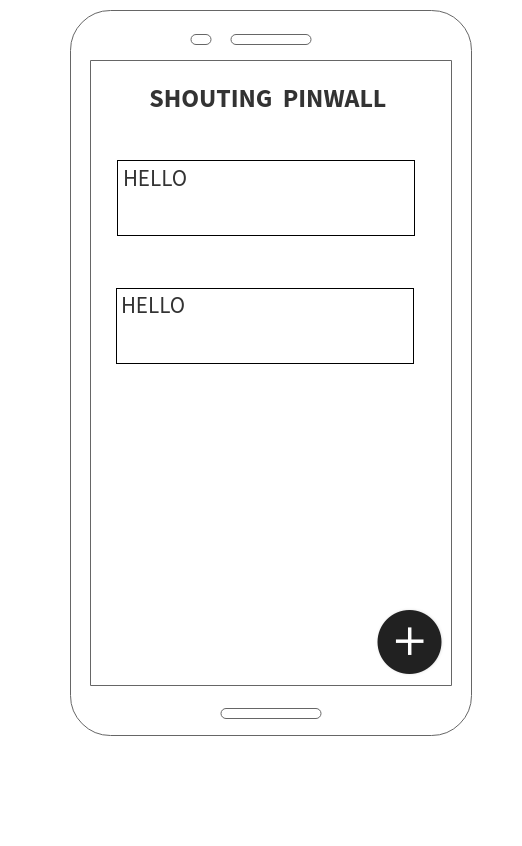
\includegraphics[width=5cm]{bibtex/images/Home_Screen.png}
\end{center}

\subsection{Add Post Screen}
This screen is for editing new post and upload it. On the top left it has text box for the post's title, and beneath it there is also a text box for the content. On the bottom, there are 'CANCEL' and 'ADD' button. 'CANCEL' button discards everything written above and brings back to Main screen. 'ADD' button completes post editing and uploads post data to the server.\\

\begin{center}
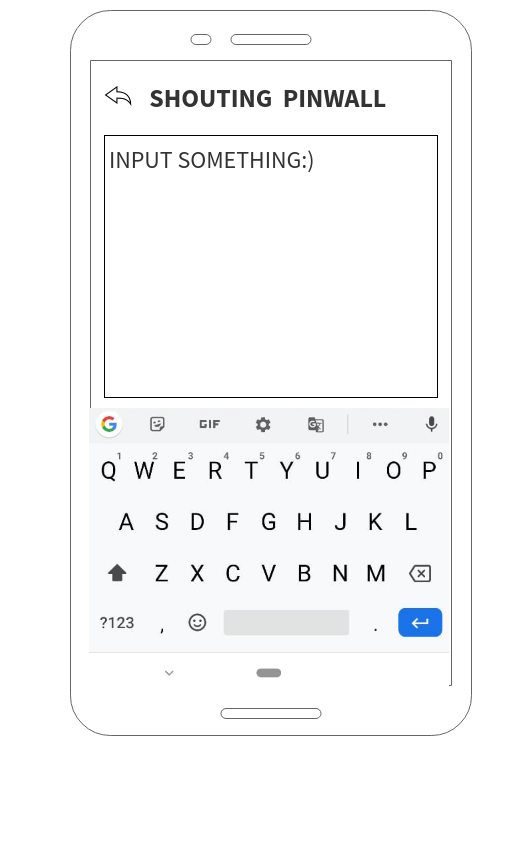
\includegraphics[width=5cm]{bibtex/images/Add_Post_Screen.png}
\end{center}

\subsection{View Post Screen}
When clicking on a post on the Main screen, this screen opens. It shows the title at the top and content below in a bigger view. In the future here could be added more details such as pictures.\\

\begin{center}
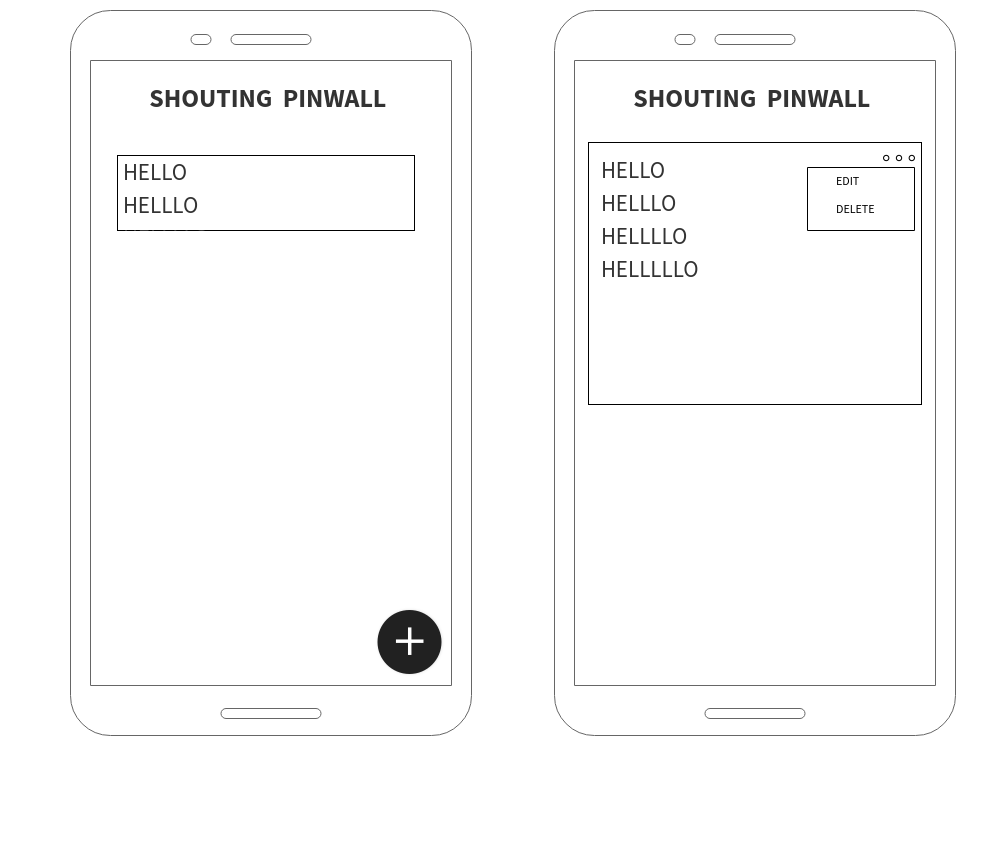
\includegraphics[width=9cm]{bibtex/images/Post_Viewing_Screen.png}
\end{center}


\section{Architecture Design}
\subsection{Overall System Architecture}
SHOUTING-PINWALL is set together with two modules. The frontend is an Android App and provides access for users and communicates with the back-end through the Firebase API from Google including encryption of the data. It's responsability is to make sure the user has easy and reliable access to the application and also handling the data.\\

The back-end stores the data it gets from the application. Firebase is a part of the Google Cloud plattform, comparable to amazons AWS. Android and Firebase are both developed by google, are very well compatible and even provide integrated encryption. We tried to get a back-end with amazon AWS to work for quite a while, but it seems to be impossible with a student account and it's restrictions and we had to give up. The Google cloud service also allows integration of analytics, functions, IAM, etc., which would be possible exteionsions for our project.\\


\begin{figure}[h]
    \centering
    \hfill
    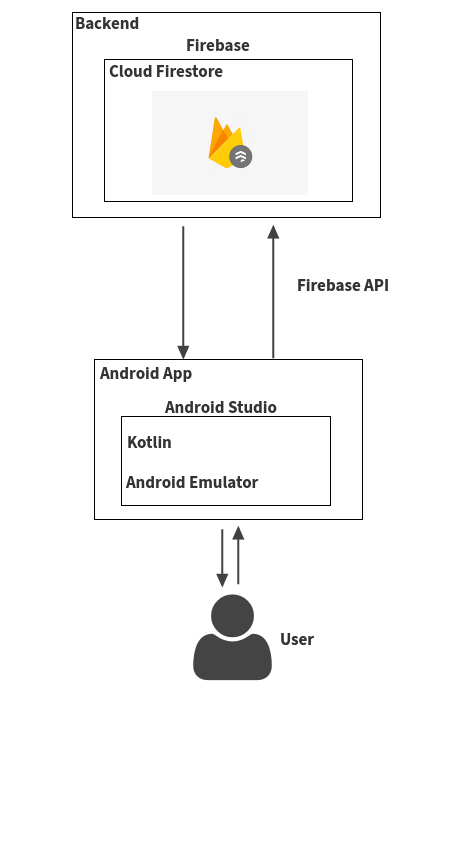
\includegraphics[width=6.5cm]
    {bibtex/images/Overall Architecture.png}
    \hfill
    \caption{Overall System Architecture}
\end{figure}



\clearpage
\subsection{Directory Organization}
huguhgutyftyf f yc trc÷÷
\\ \hspace*{\fill} \\


\begin{table}[]
    \caption{Directory Organization}
    \begin{tabular}{|c|c|c|}
    \hline
    Directory & File Name & Module Name \\ \hline
    Pinwall/app/main & \begin{tabular}[c]{@{}c@{}}AddPostActivity.kt \\ ListAdapater.kt \\ MainActivity.kt \\ Post.kt\\ PostComperator.kt\end{tabular} & Android App \\ \hline
    Pinwall/app/res/drawable & \begin{tabular}[c]{@{}c@{}}add.png\\ men.png\\ women.png\end{tabular} & Android App \\ \hline
    Pinwall/app/res/layout & \begin{tabular}[c]{@{}c@{}}activity\_add\_post.xml\\ activity\_main.xml\\ list\_item.xml\end{tabular} & Android App \\ \hline
    Pinwall/app/res/mipmap-hdpi & \begin{tabular}[c]{@{}c@{}}ic\_launcher.png\\ ic\_launcher\_round.png\end{tabular} & Android App \\ \hline
    Pinwall/app/res/mipmap-mdpi & \begin{tabular}[c]{@{}c@{}}ic\_launcher.png\\ ic\_launcher\_round.png\end{tabular} & Android App \\ \hline
    Pinwall/app/res/mipmap-xhdpi & \begin{tabular}[c]{@{}c@{}}ic\_launcher.png\\ ic\_launcher\_round.png\end{tabular} & Android App \\ \hline
    Pinwall/app/res/mipmap-xxhdpi & \begin{tabular}[c]{@{}c@{}}ic\_launcher.png\\ ic\_launcher\_round.png\end{tabular} & Android App \\ \hline
    Pinwall/app/res/mipmap-xxxhdi & \begin{tabular}[c]{@{}c@{}}ic\_launcher.png\\ ic\_launcher\_round.png\end{tabular} & Android App \\ \hline
    Pinwall/app/res/values & \begin{tabular}[c]{@{}c@{}}colors.xml\\ strings.xml\\ themes.xml\end{tabular} & Android App \\ \hline
    Pinwall/app/res/values-night & themes.xml & Android App \\ \hline
    Pinwall/doc & \begin{tabular}[c]{@{}c@{}}SHOUTING\\ PINWALL.tex\end{tabular} & Documentation \\ \hline
    \end{tabular}
    \end{table}


\section{Classes}
\subsection{AddPostActivity.kt}
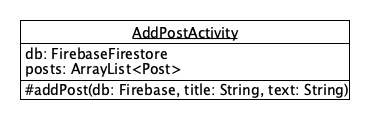
\includegraphics[width = 8cm]{bibtex/images/AddPostActivity.png}
\begin{enumerate}
    \item The var 'db' is responsible for handling database and provides function such as storing and loading data from firebase server.
    \item addBttn in this class triggers action of uploading title and text data to database 'db.'
\end{enumerate}

\subsection{ListAdapter.kt}
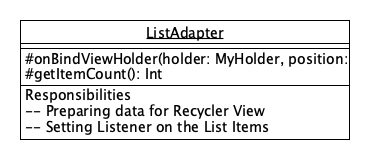
\includegraphics[width = 8cm]{bibtex/images/ListAdapter.png}
\begin{enumerate}
    \item This class includes controls how list of posts are displayed on main screen, by using recyclerview. It fetches 'title' and 'text' data and displays as "listitem.xml" design.
\end{enumerate}

\subsection{MainActivity.kt}
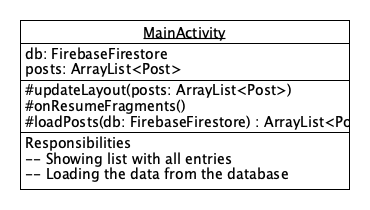
\includegraphics[width = 8cm]{bibtex/images/MainActivity.png}
\begin{enumerate}
    \item posts
    \begin{enumerate}
        \item this is array of data from Post.kt which includes 'title', 'text' and 'timestamp' data.
    \end{enumerate}
    \item updateLayout()
        \begin{enumerate}
            \item This function loads latest data from the server on starting the app.
        \end{enumerate}
    \item loadPosts()
        \begin{enumerate}
            \item This function is responsible for loading post data from the server.
        \end{enumerate}
    \item onResumeFragments()
        \begin{enumerate}
            \item This function allows the app to automatically refresh after returning from other intent such as 'AddPostActivity'
        \end{enumerate}
\end{enumerate}

\subsection{Post.kt}
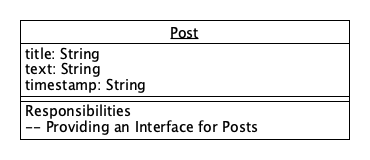
\includegraphics[width = 8cm]{bibtex/images/Post.png}
\begin{enumerate}
    \item title
        \begin{enumerate}
            \item Contains String data of what user wrote on 'ap-titleBox' textbox.
        \end{enumerate}
    \item text
        \begin{enumerate}
            \item Contains String data of what user wrote on 'ap-textBox' textbox.
        \end{enumerate}
    \item timestamp
        \begin{enumerate}
            \item Contains String data of timestamp when user uploads his/her post on the server.
        \end{enumerate}
\end{enumerate}


\subsection{PostComperator.kt}
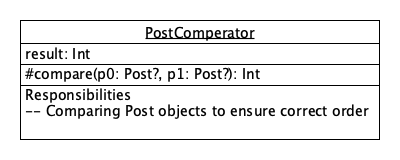
\includegraphics[width = 8cm]{bibtex/images/PostComperator.png}
\begin{enumerate}
    \item By default Posts are sorted by the ID, which is a randomly generated value by firebase. As a result the posts are sorted in a random order. To fix this and order the items by the time added, we added a timestamp to the posts and created this comperator.
\end{enumerate}





\section{Use Cases}
\subsection{Adding Post}
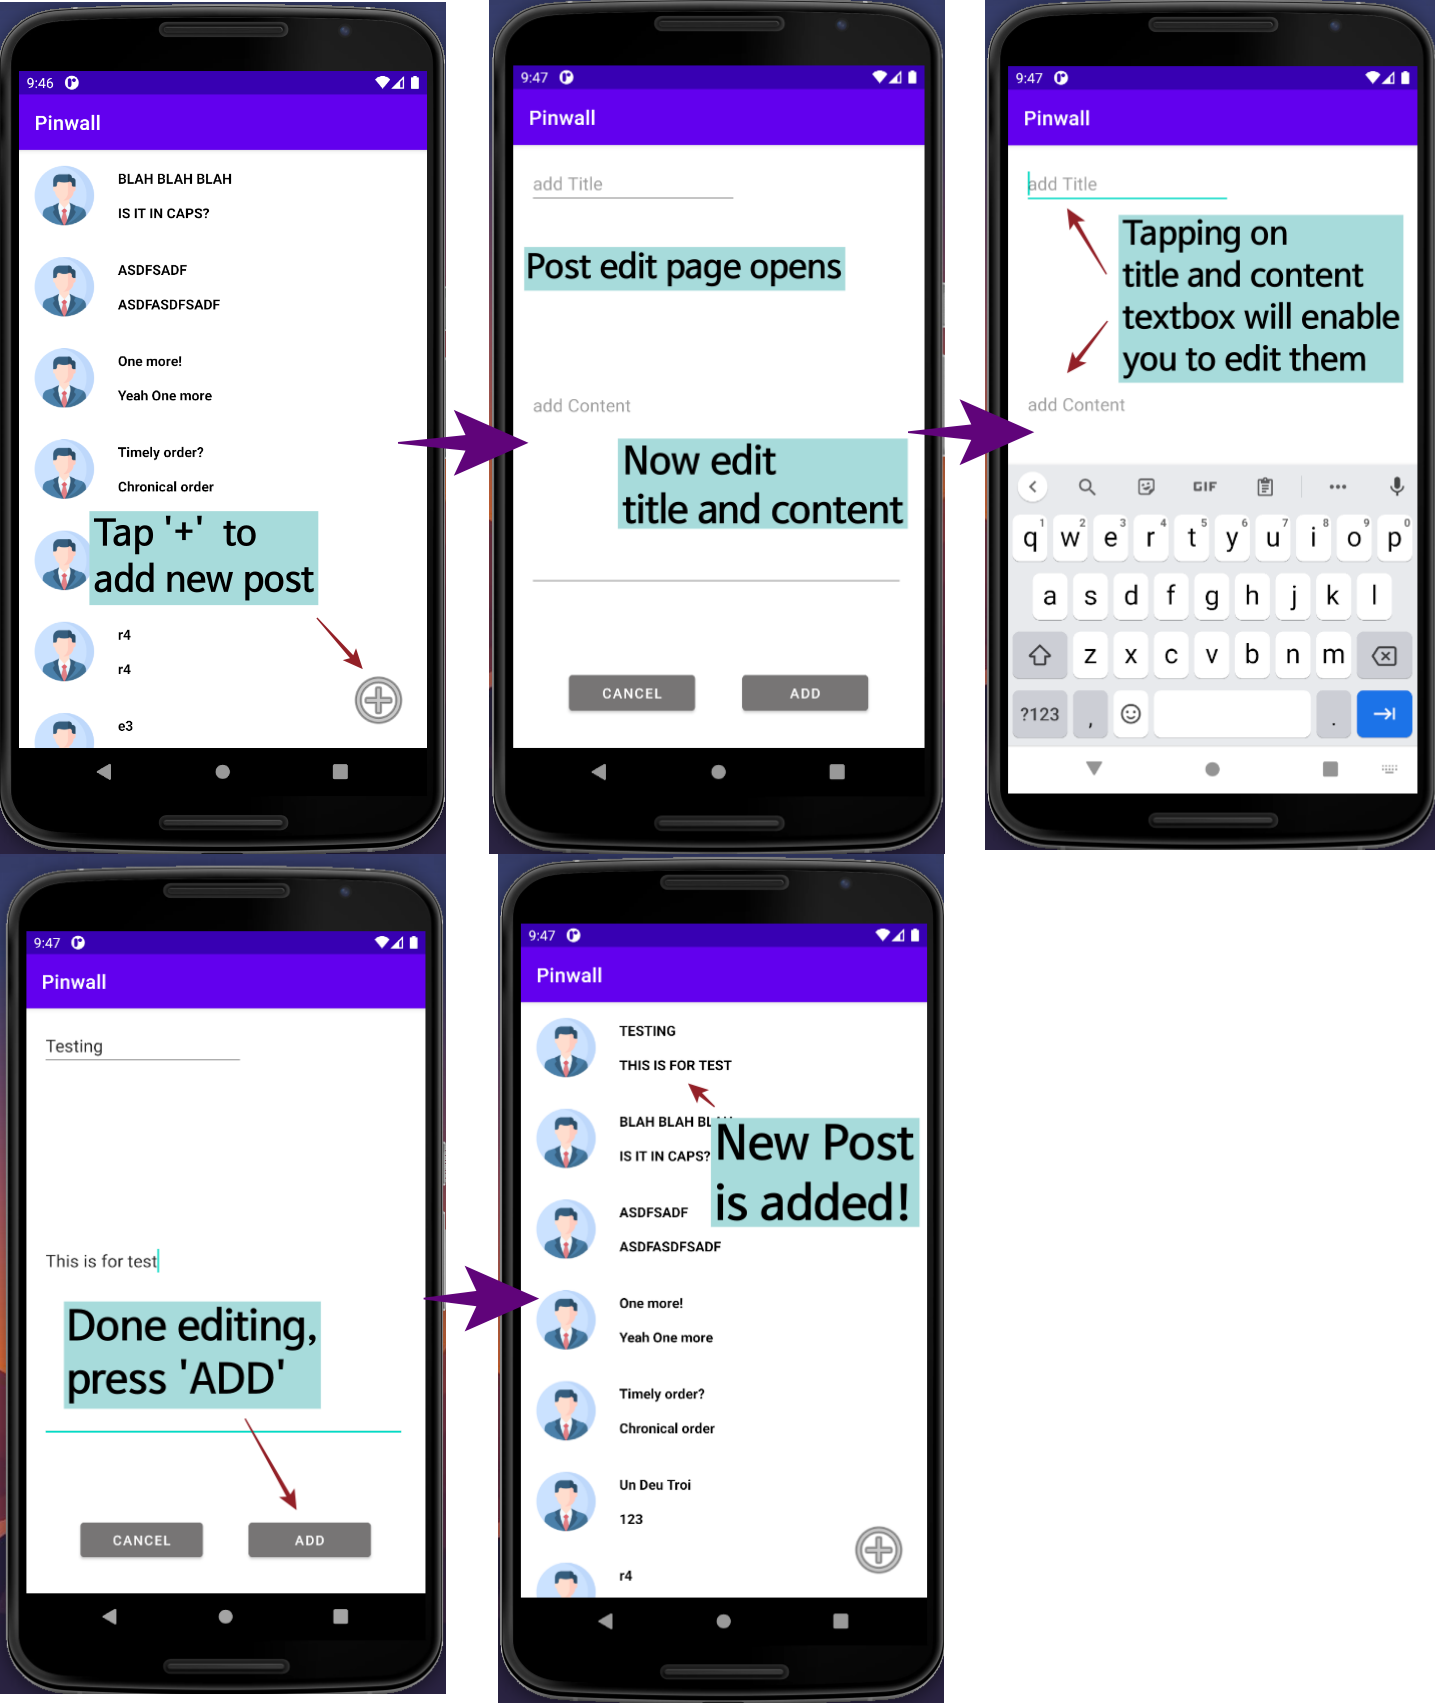
\includegraphics[width = 8cm]{bibtex/images/use case 1.png}

\subsection{Updating Post list}
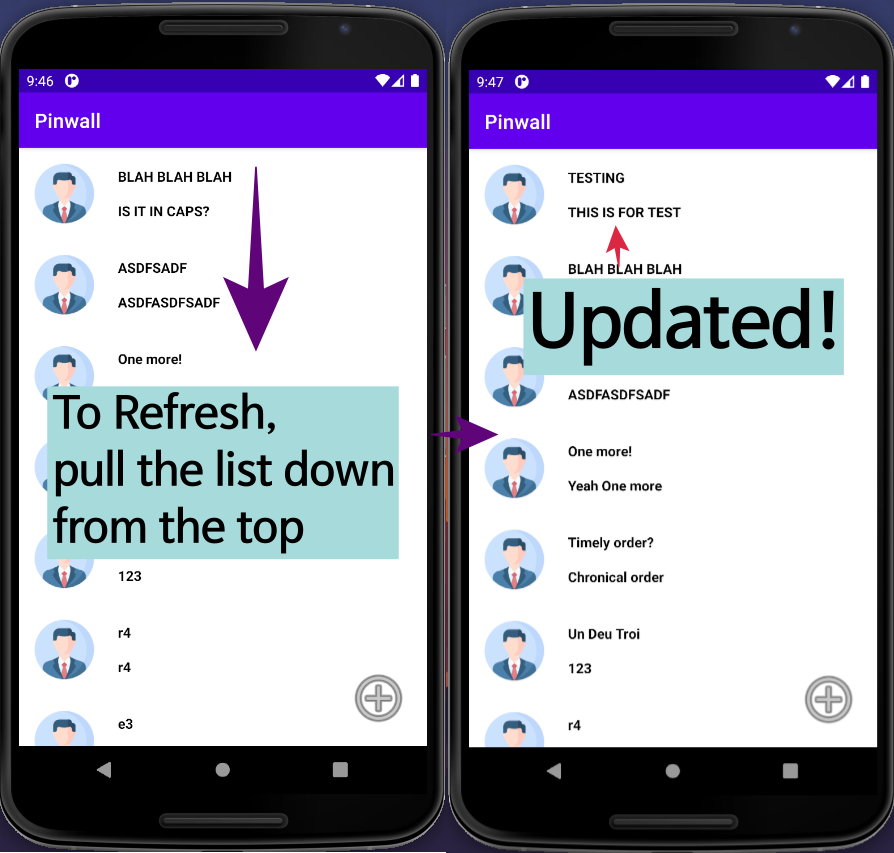
\includegraphics[width = 7cm]{bibtex/images/use case 2.png}

\subsection{Discard New post}
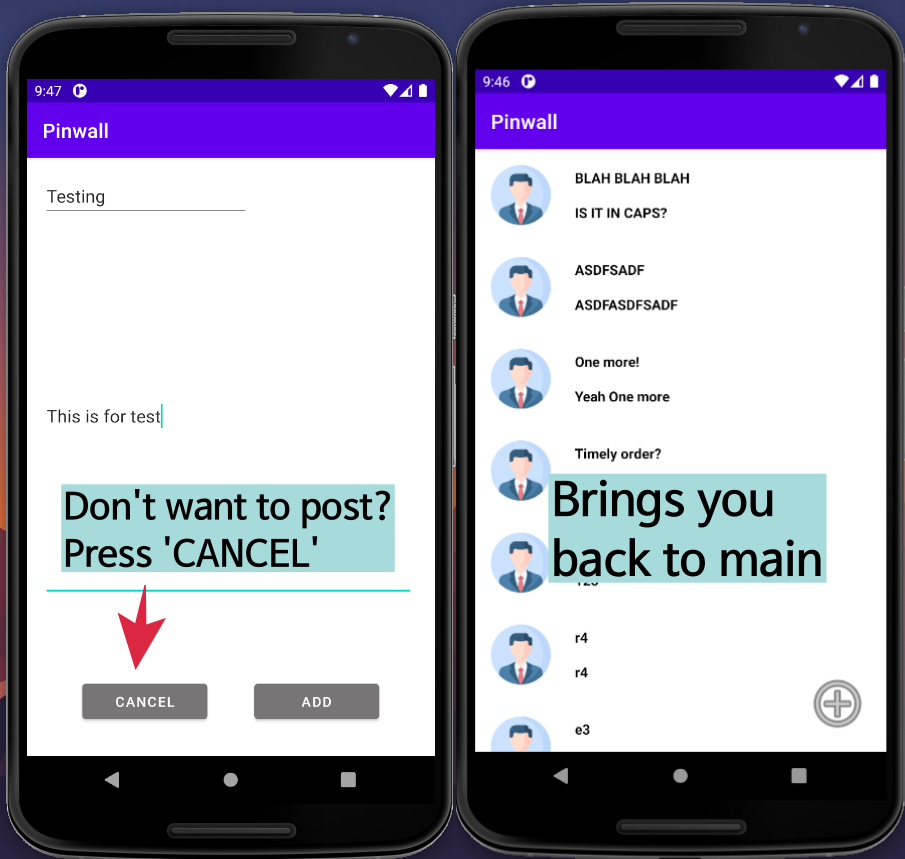
\includegraphics[width = 7cm]{bibtex/images/use case 3.png}


\end{document}